\chapter[Requerimientos de red - Hardware]{Requerimientos de red - Hardware}
\label{cp:requerimientos-hardware}
{

\section*{Resumen}
Este capítulo detalla la infraestructura física de red y el hardware de los cinco espacios usados por los laboratorios de enseñanza del Departamento de Física. Se documenta la distribución de los recursos, incluyendo la ubicación de los switches, las bocas de red requeridas por espacio (para computadoras, periféricos y equipos de medición) y las especificaciones del equipamiento asignado a alumnos, docentes y pañol.

El propósito de este relevamiento es servir como referencia para el personal técnico y de IT. Al mapear la topología física y el inventario, se busca facilitar la identificación de conexiones, agilizar el mantenimiento y aportar información de apoyo para la migración de los servidores.

\section{Red física}
Esta sección documenta la disposición física del cableado en cada espacio mediante planos que indican la ubicación de los switches y las bocas de red. 

Para facilitar el rastreo de las conexiones, los planos incluyen la numeración de las computadoras y se complementan con una tabla de mapeo que especifica a qué switch corresponde cada boca. Esta referencia visual y estructurada busca simplificar la identificación rápida del cableado durante las tareas de mantenimiento.

\subsection{Laboratorio 1}
\begin{figure}[H]
    \centering
    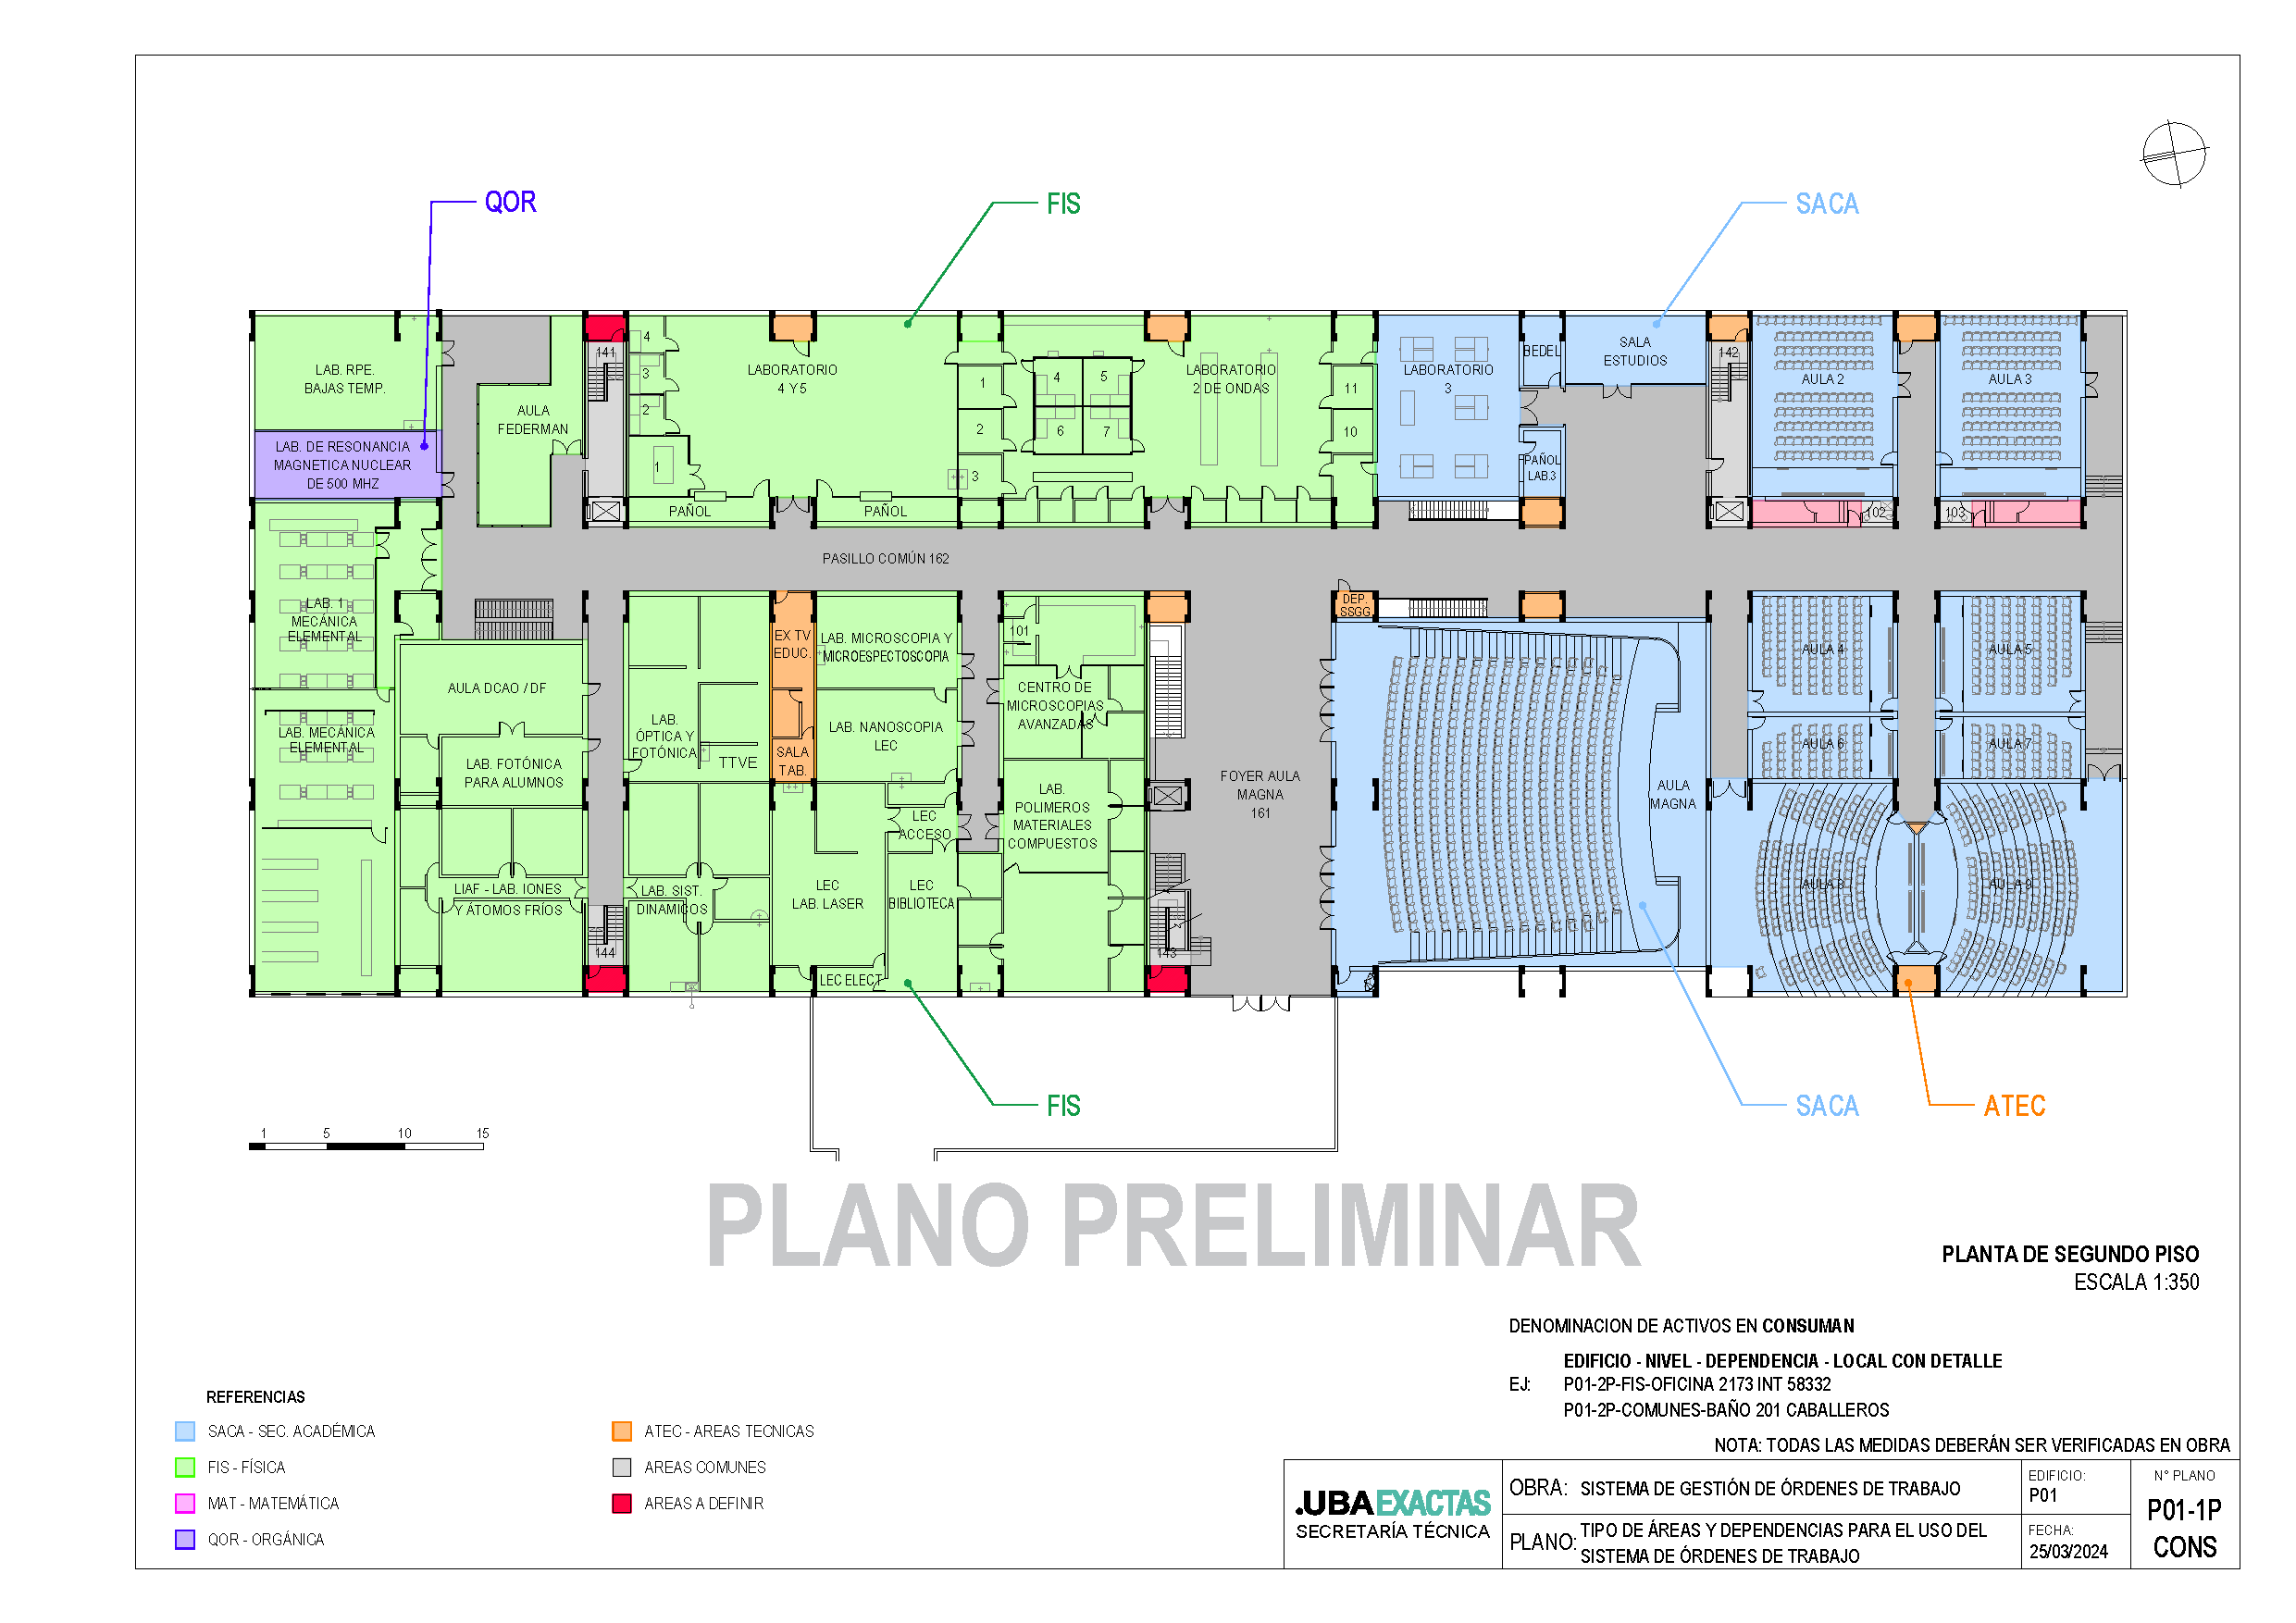
\includegraphics[width=0.8\textwidth]{Figuras/planos/P01-1P-CONS-PRELIMINAR.pdf}
    \caption{Infraestructura de computación del laboratorio 1 - editar plano para reflejar el espacio en cuestión}
    \label{fig:it-fisico-l1}
\end{figure}
\subsection{Laboratorio 2}
\begin{figure}[H]
    \centering
    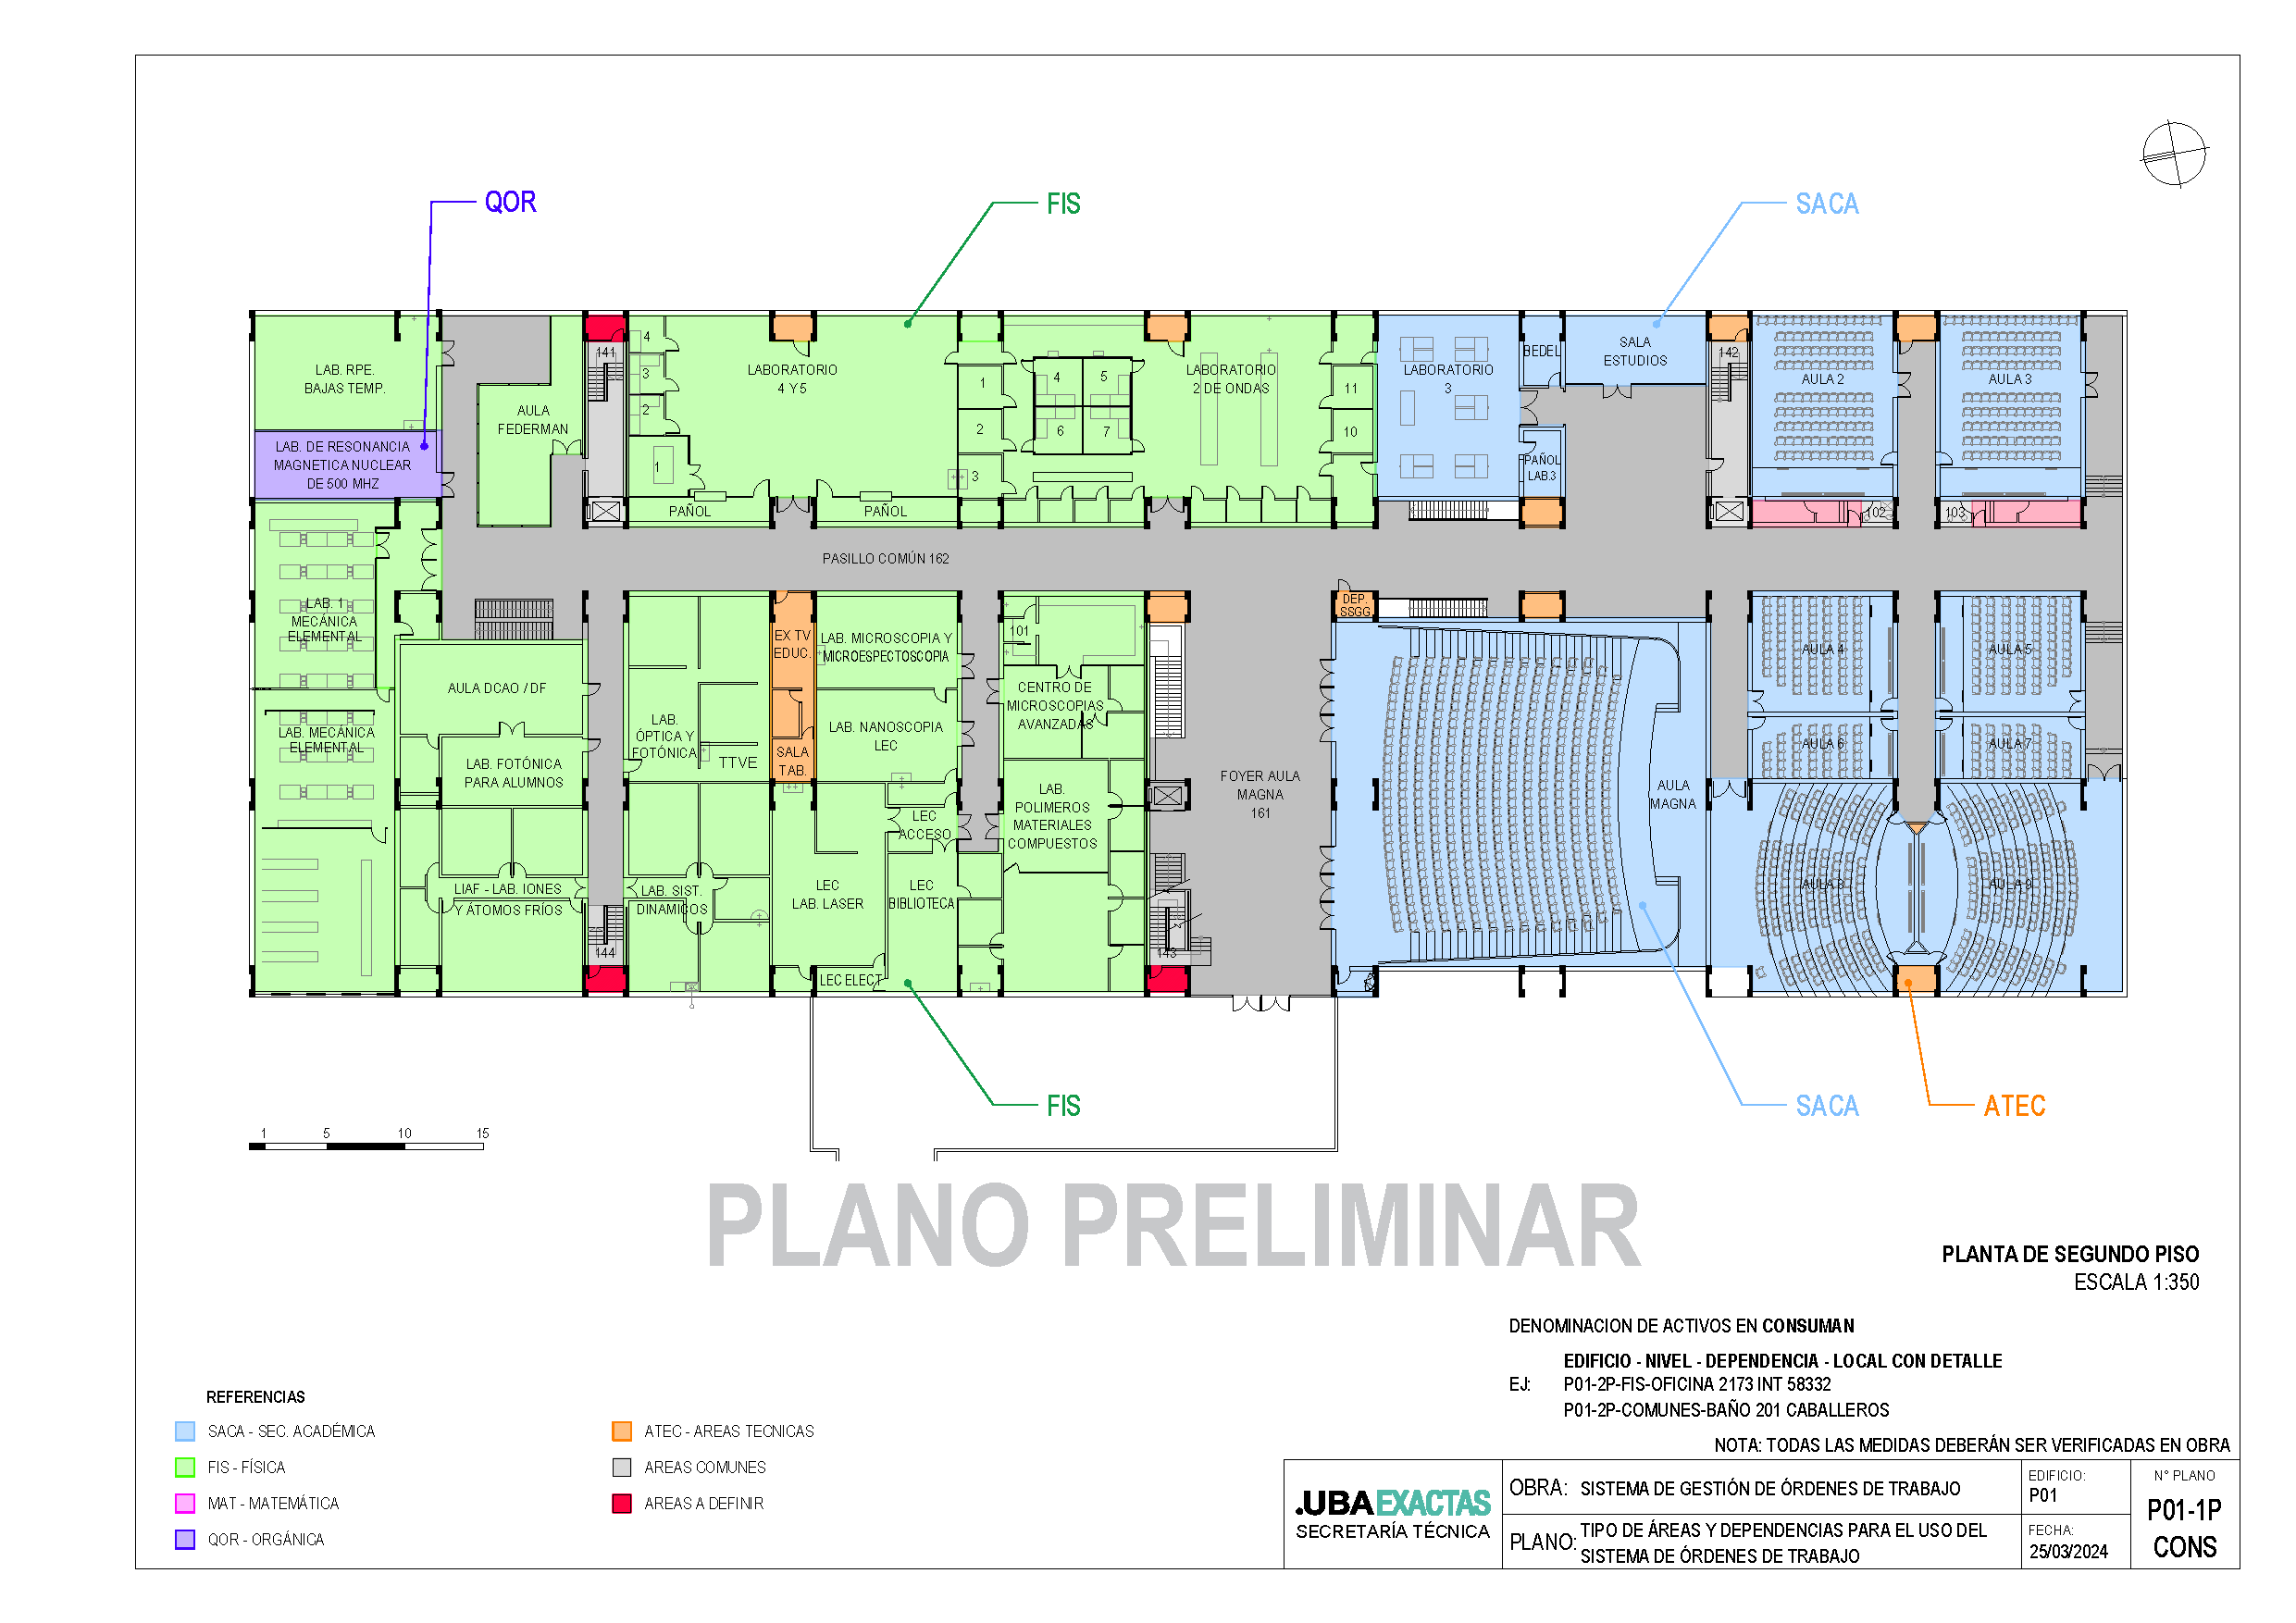
\includegraphics[width=0.8\textwidth]{Figuras/planos/P01-1P-CONS-PRELIMINAR.pdf}
    \caption{Infraestructura de computación del laboratorio 2 - editar plano para reflejar el espacio en cuestión}
    \label{fig:it-fisico-l2}
\end{figure}
\subsection{Laboratorio 3}
\begin{figure}[H]
    \centering
    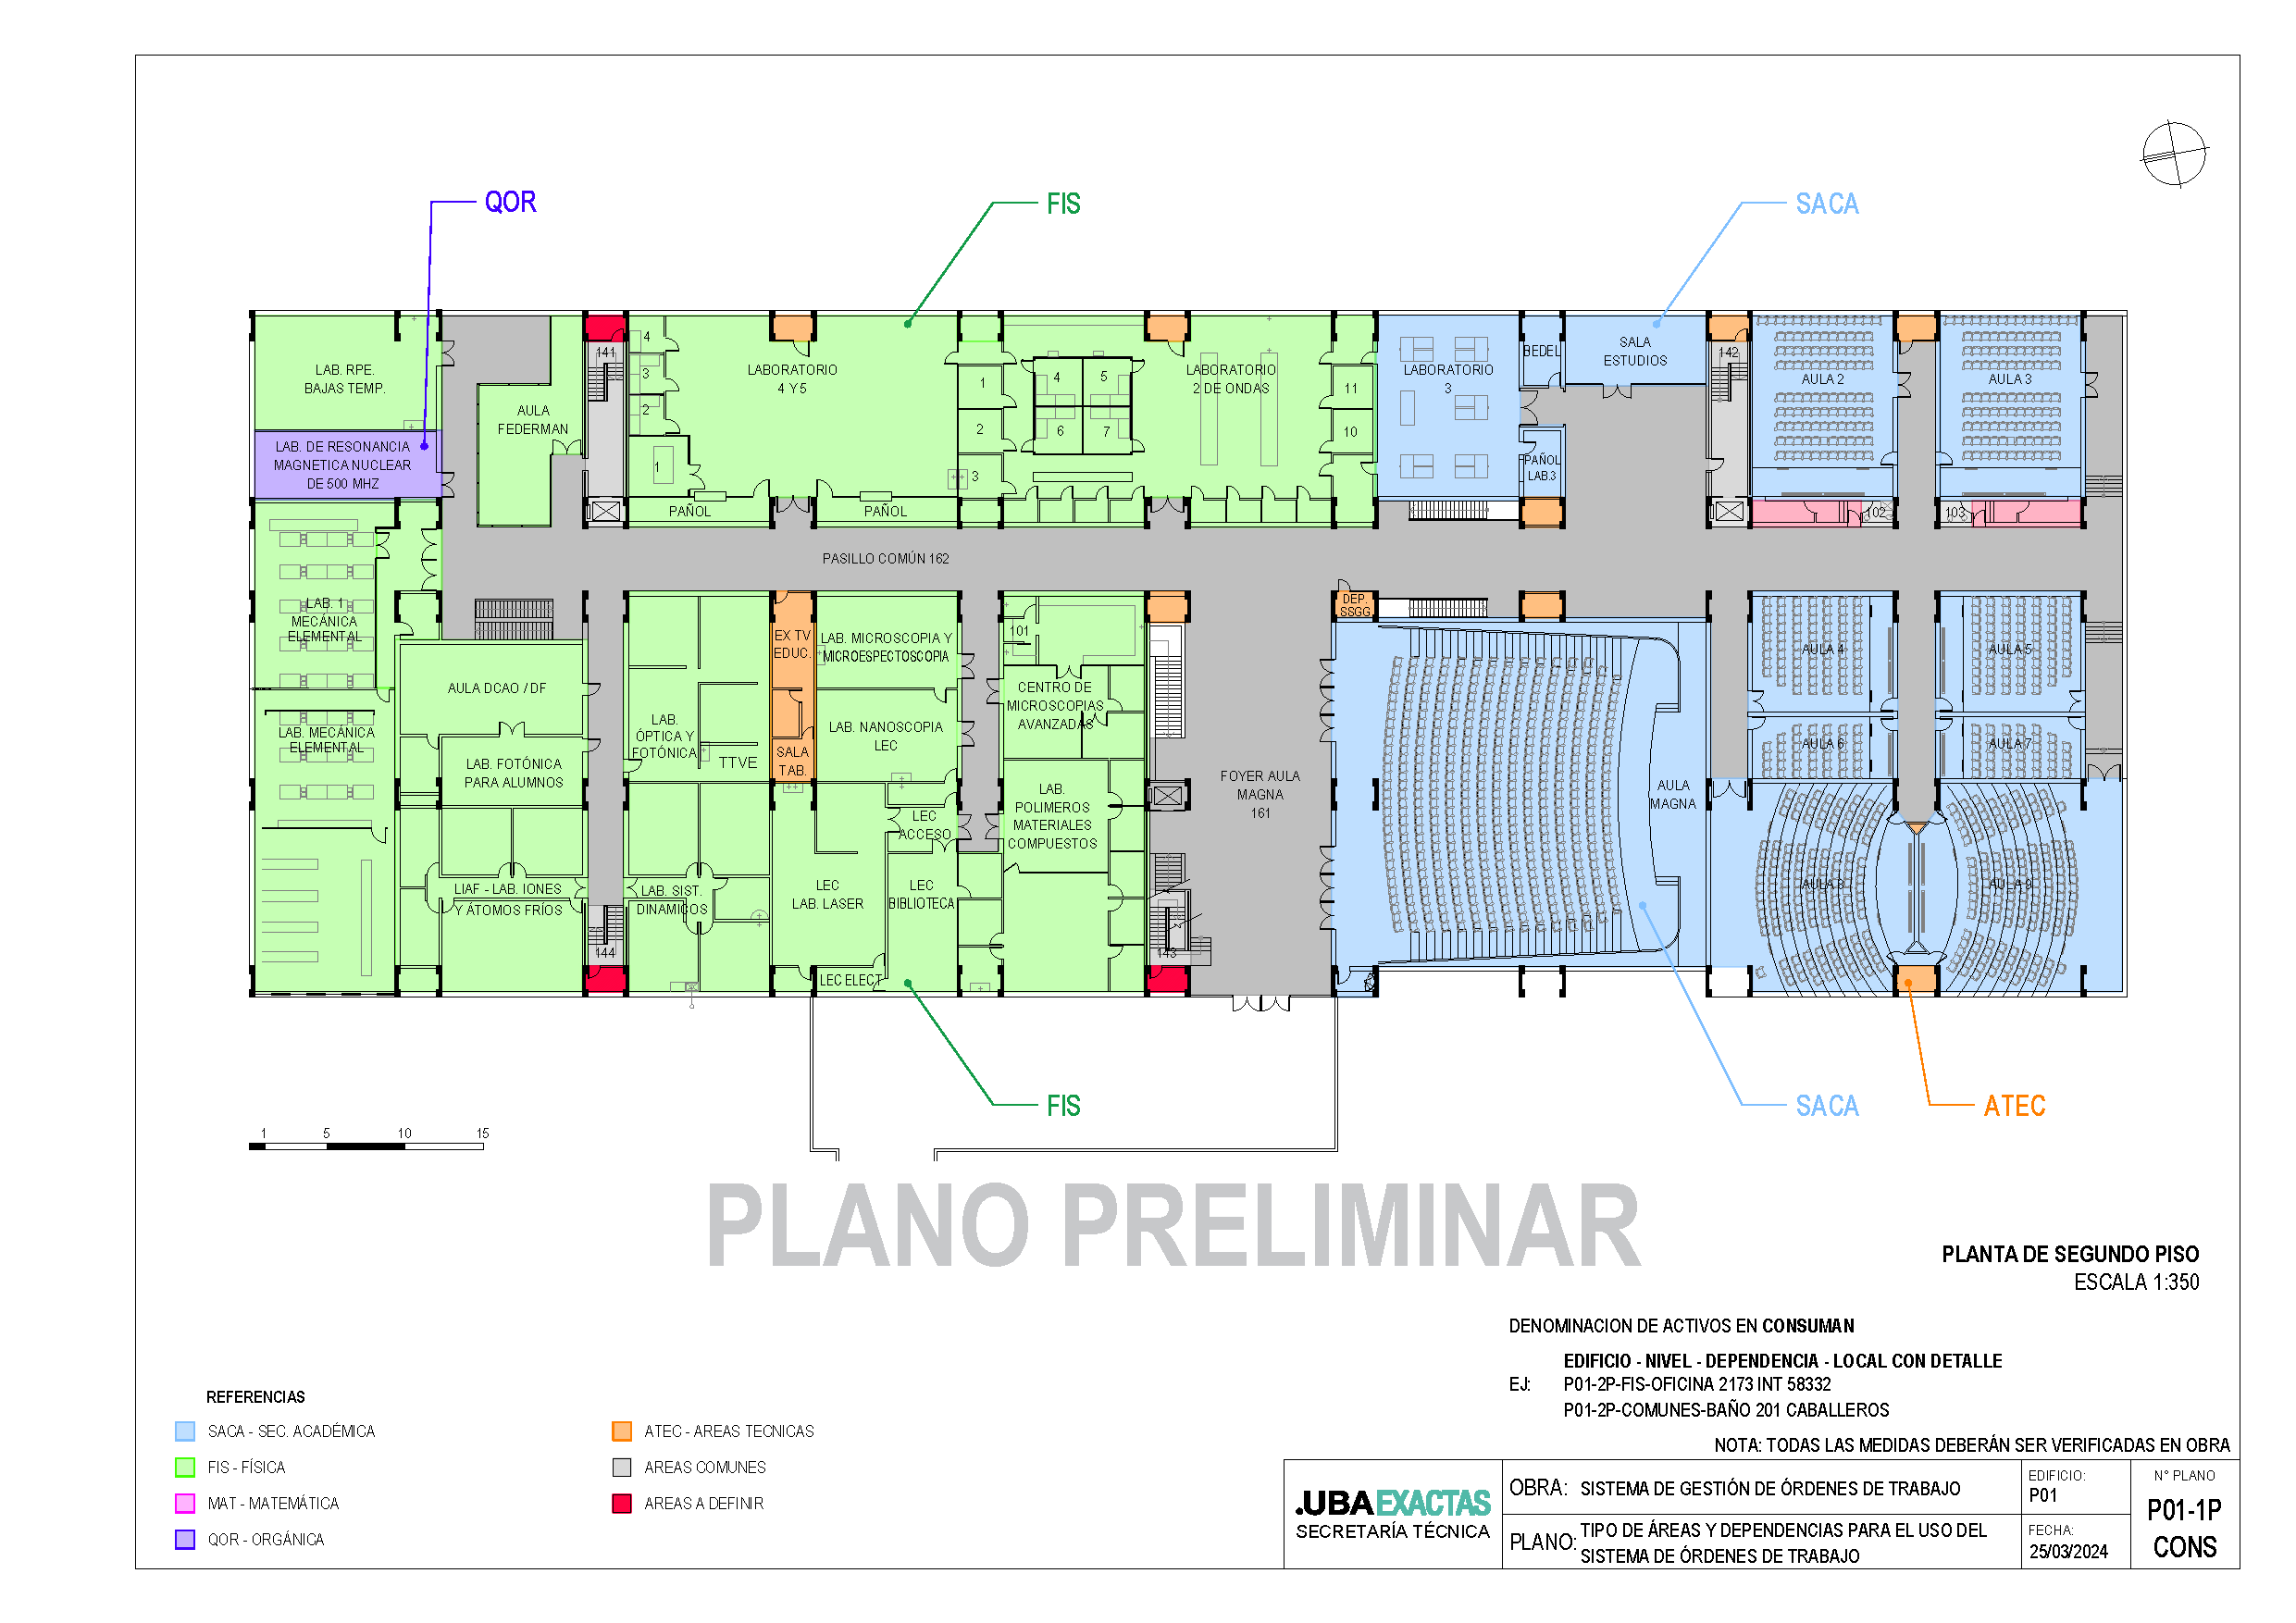
\includegraphics[width=0.8\textwidth]{Figuras/planos/P01-1P-CONS-PRELIMINAR.pdf}
    \caption{Infraestructura de computación del laboratorio 3 - editar plano para reflejar el espacio en cuestión}
    \label{fig:it-fisico-l3}
\end{figure}
\subsection{Laboratorios avanzados}
\begin{figure}[H]
    \centering
    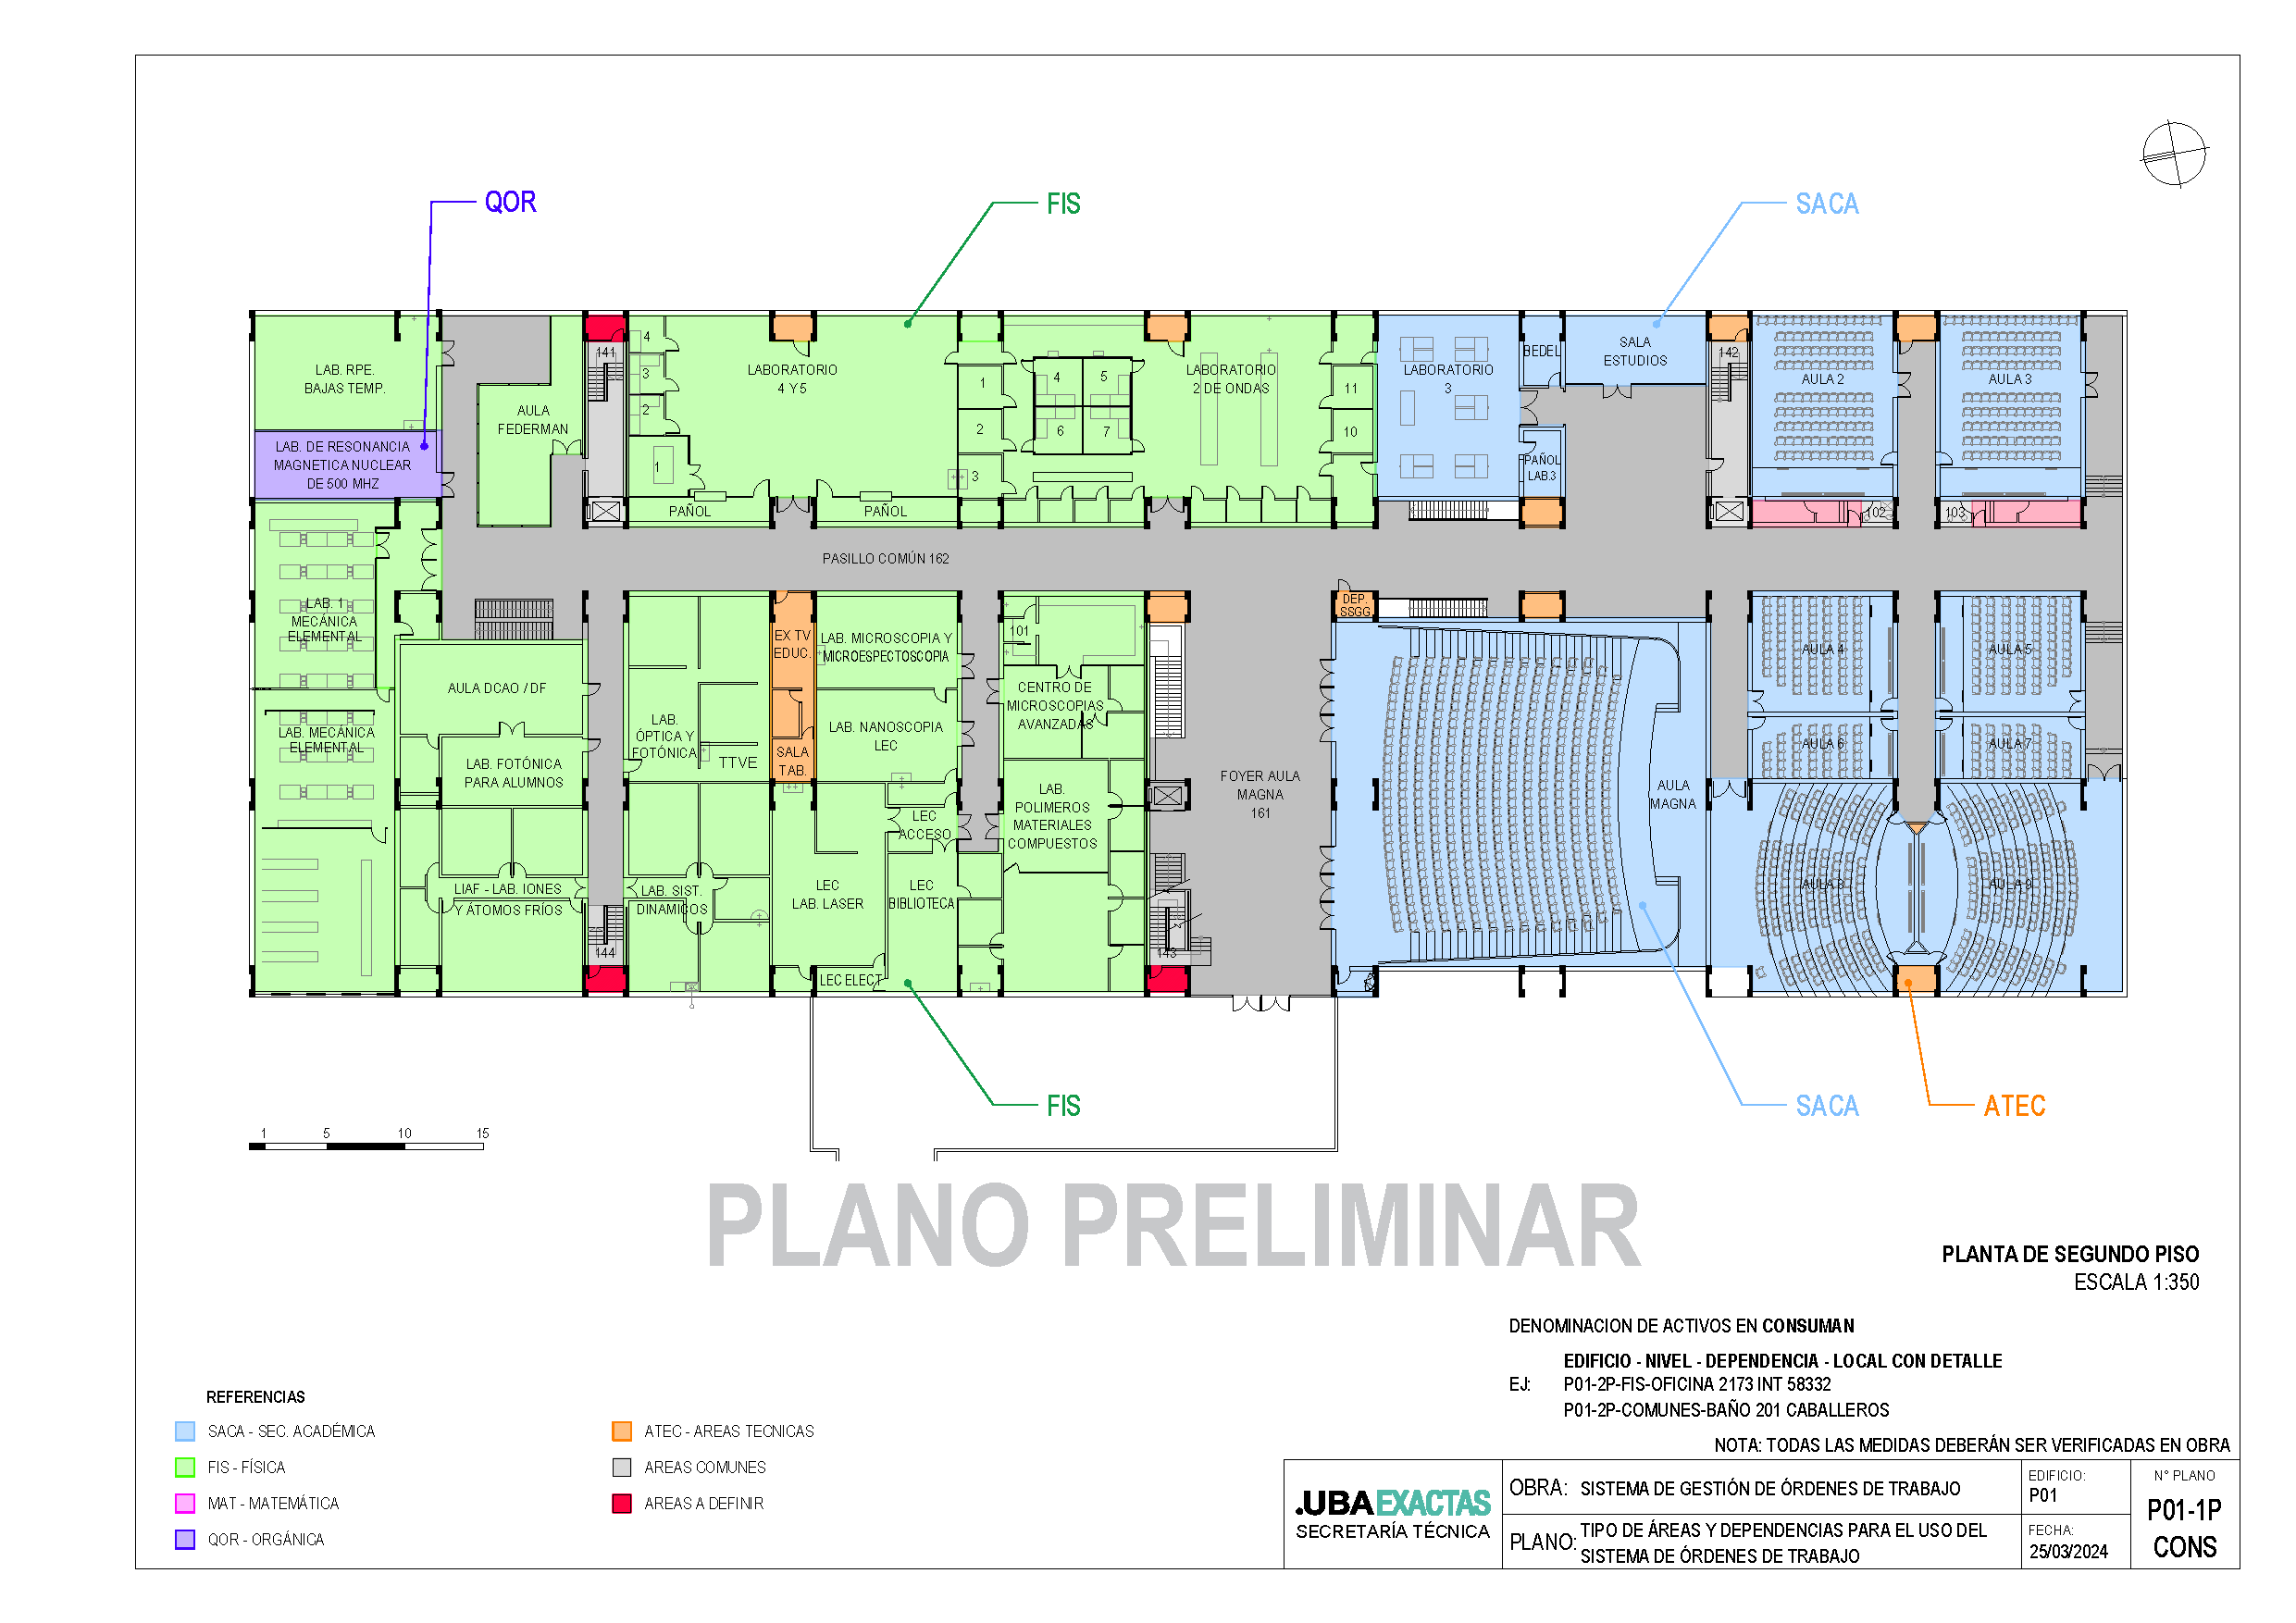
\includegraphics[width=0.8\textwidth]{Figuras/planos/P01-1P-CONS-PRELIMINAR.pdf}
    \caption{Infraestructura de computación del laboratorio avanzado de física - editar plano para reflejar el espacio en cuestión}
    \label{fig:it-fisico-la}
\end{figure}
\subsection{Laboratorio de Fotónica}
\begin{figure}[H]
    \centering
    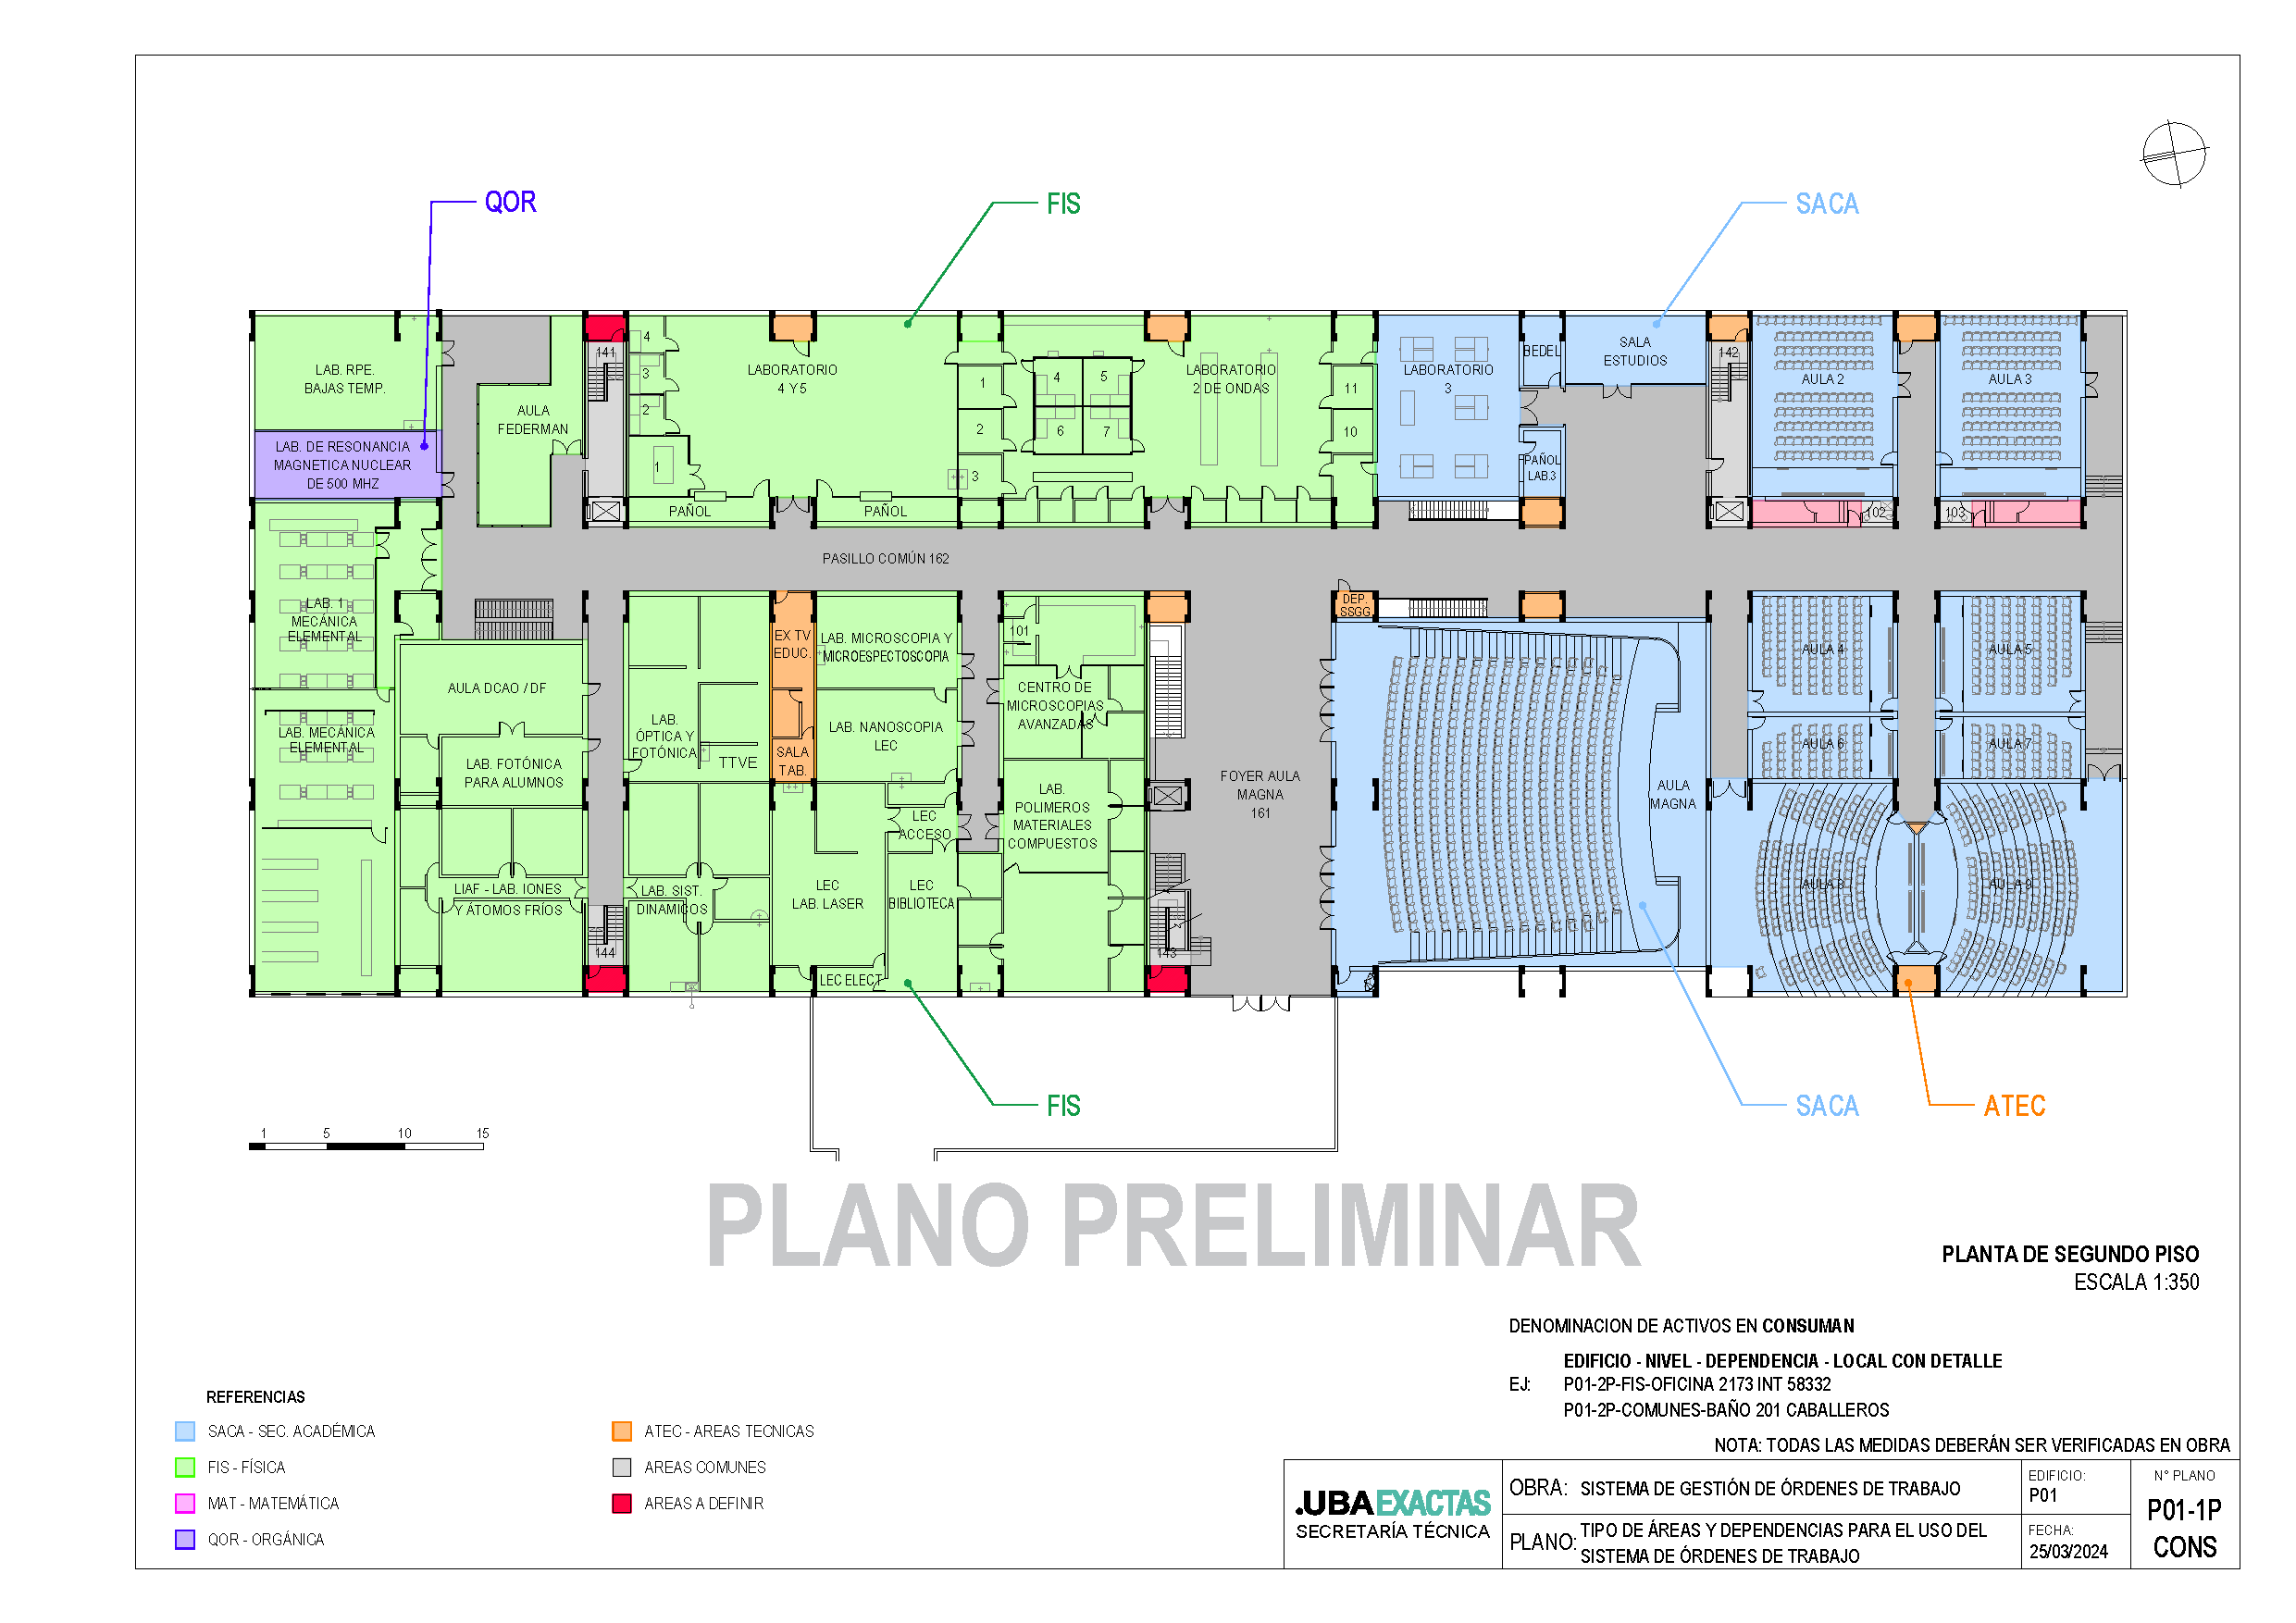
\includegraphics[width=0.8\textwidth]{Figuras/planos/P01-1P-CONS-PRELIMINAR.pdf}
    \caption{Infraestructura de computación del laboratorio de Fotónica - editar plano para reflejar el espacio en cuestión}
    \label{fig:it-fisico-lf}
\end{figure}

\section{Hardware}
Esta sección detalla el inventario y las especificaciones de las computadoras de cada espacio, agrupadas según su usuario (alumnos, docentes y pañol). 

Se documenta la cantidad de terminales y las imágenes de sistema asociadas al rol de cada una. Este listado busca servir como referencia rápida para conocer la distribución de los equipos y brindar información de apoyo para futuras clonaciones o tareas de mantenimiento.

\subsection{Laboratorio 1}
\paragraph{Alumnos} 14 computadoras de alumnos con:
\begin{itemize}
    \item \textbf{Procesador} Intel i5 -----
    \item ---
    \item Imagen del sistema L1A-IMG001-2026 (referencia a la imagen real actual)
\end{itemize}

\paragraph{Docentes} 1 computadora para docentes con:
\begin{itemize}
    \item \textbf{Procesador} Intel i5 -----
    \item ---
    \item Imagen del sistema L1D-IMG001-2026 (referencia a la imagen real actual)
\end{itemize}

\paragraph{Pañol} 1 computadora para técnicos con:
\begin{itemize}
    \item \textbf{Procesador} Intel i5 -----
    \item ---
    \item Imagen del sistema L1P-IMG001-2026 (referencia a la imagen real actual)
\end{itemize}

\subsection{Laboratorio 2}
\paragraph{Alumnos} 12 computadoras de alumnos con:
\begin{itemize}
    \item \textbf{Procesador} Intel i5 -----
    \item ---
    \item Imagen del sistema L2A-IMG001-2026 (referencia a la imagen real actual)
\end{itemize}

\paragraph{Docentes} 1 computadora para docentes con:
\begin{itemize}
    \item \textbf{Procesador} Intel i5 -----
    \item ---
    \item Imagen del sistema L2D-IMG001-2026 (referencia a la imagen real actual)
\end{itemize}

\paragraph{Pañol} 1 computadora para técnicos con:
\begin{itemize}
    \item \textbf{Procesador} Intel i5 -----
    \item ---
    \item Imagen del sistema L2P-IMG001-2026 (referencia a la imagen real actual)
\end{itemize}

\subsection{Laboratorio 3}
\paragraph{Alumnos1} 10 computadoras de alumnos con:
\begin{itemize}
    \item \textbf{Procesador} Intel i5 -----
    \item ---
    \item Imagen del sistema L3A-IMG001-2026 (referencia a la imagen real actual)
\end{itemize}

\paragraph{Alumnos2} 2 computadoras de alumnos con:
\begin{itemize}
    \item \textbf{Procesador} Intel i5 -----
    \item ---
    \item Imagen del sistema LAA-IMG002-2026 (referencia a la imagen real actual)
\end{itemize}

\paragraph{Docentes} 1 computadora para docentes con:
\begin{itemize}
    \item \textbf{Procesador} Intel i5 -----
    \item ---
    \item Imagen del sistema L3D-IMG001-2026 (referencia a la imagen real actual)
\end{itemize}

\paragraph{Pañol} 1 computadora para técnicos con:
\begin{itemize}
    \item \textbf{Procesador} Intel i5 -----
    \item ---
    \item Imagen del sistema L3P-IMG001-2026 (referencia a la imagen real actual)
\end{itemize}

\subsection{Laboratorio 4}

\paragraph{Alumnos} 14 computadoras de alumnos con:
\begin{itemize}
    \item \textbf{Procesador} Intel i5 -----
    \item ---
    \item Imagen del sistema LAA-IMG001-2026 (referencia a la imagen real actual)
\end{itemize}

\paragraph{Docentes} 1 computadora para docentes con:
\begin{itemize}
    \item \textbf{Procesador} Intel i5 -----
    \item ---
    \item Imagen del sistema LAD-IMG001-2026 (referencia a la imagen real actual)
\end{itemize}

\paragraph{Pañol} 1 computadora para técnicos con:
\begin{itemize}
    \item \textbf{Procesador} Intel i5 -----
    \item ---
    \item Imagen del sistema LAP-IMG001-2026 (referencia a la imagen real actual)
\end{itemize}

\subsection{Laboratorio de Fotónica}

\paragraph{Alumnos} 2 computadoras de alumnos con:
\begin{itemize}
    \item \textbf{Procesador} Intel i5 -----
    \item ---
    \item Imagen del sistema LFA-IMG001-2026 (referencia a la imagen real actual)
\end{itemize}

}